\documentclass[12 pt]{article}

\usepackage[utf8]{inputenc}
\usepackage[ngerman]{babel}

\usepackage{graphicx}
\usepackage[absolute]{textpos}

\usepackage{hyperref}
\usepackage[nameinlink]{cleveref}
\crefname{figure}{Abb.}{Abb.}

\usepackage{pflichtenheft}
\begin{document}
	
	%TODO
	\subsection{Produktübersicht}
	
	Der \textbf{FR}aunhofer\textbf{O}penSource\textbf{S}ensor\textbf{T}ings-Server des Fraunhofer IOSB ist eine Open-Source-Implementierung des SensorThings-Standards des OGC und unter https://github.com/FraunhoferIOSB/FROST-Server downloadbar.
	\\ \\ Der FROST-Server dient der Speicherung und Verwaltung von Sensordaten.\\
	Unsere Software stellt zu diesem Server eine einfache und dennoch stark konfigurierbare Weboberfläche bereit, die es ermöglicht Sensordaten aus einer Tabelle einzulesen, zu konvertieren und auf einen FROST-Server zu übertragen. 
	\\ \\Die Software läuft in einer Java JRE und das zugehörige Webinterface soll über einen herkömmlichen PC, einen Laptop oder ein Tablet erreichbar sein.\\
	Sie ist ebenfalls Open-Source und soll überall dort eingesetzt werden, wo Daten aus Tabellen importiert, konvertiert und auf den FROST-Server übertragen werden sollen. \\
	\\Hierzu zählt:
	\begin{itemize}
		\item Der Import von neuen Sensordaten, welche in CSV-/XSLX-Tabellen-Form vorliegen
		\item Die Integration von bestehenden (archivierten) Sensordaten, welche in CSV-/XLSX-Tabellen-Form vorliegen
	\end{itemize}
	
	\subsection{Musskriterien}
\begin{enumerate}
	\item Import von Daten \\
	Die Daten sollen aus Tabellen im CSV-/Excel-Dateiformat importiert werden
	\item Konvertierung des Formats der Sensordaten \\
	Die Daten sollen aus den beliebigen Datenformaten und Anordnungen innerhalb der Quelldatei in den einheitlichen Standard der SensorThings API konvertiert werden.
	Damit entsprechen sie dem Standard der Daten auf einem FROST-Server.
	\item Erstellen, Abspeichern und Laden von Konfigurationen \\
	Der Benutzer soll Spaltenformat, Datenformat und insbesondere Datums- und Zeitformat einstellen und als Konfiguration abspeichern können.
	Diese Konfigurationen sollen später auch wieder geladen werden können.
	\item Datentyptransformationen \\
	Alle Werte sind in der Quelldatei als String vorhanden und müssen, bevor sie auf den FROST-Server geladen werden, in den passenden Datentyp (bspw. Integer) umgewandelt werden.
	Sonderwerte (Magic Numbers) sollen nicht auf den FROST-Server geladen, sondern separat behandelt werden.
\end{enumerate}

\subsection{Wunschkriterien}
\begin{enumerate}
	\item Standard-Konfiguration \\
	Dem Benutzer wird eine vorgefertigte Konfiguration bestehend aus Spaltenformat, Datenformat und Datums- und Zeitformat bereitgestellt.
	\item Überprüfung auf Duplikate \\
	Beim Upload der Daten auf den FROST-Server werden diese mit den bestehenden Daten abgeglichen und Duplikate werden nicht erneut gespeichert.
	\item Rückgabe nicht bearbeiteter Datensätze in neuer CSV-Datei \\
	Bei (teilweise) fehlgeschlagener Übertragung zum FROST-Server werden die nicht übertragenen Daten in einer CSV-Datei an den Benutzer zurückgegeben.
	\item Korrektur von falschen Daten \\
	Der Benutzer hat die Möglichkeit Fehler in den Daten direkt zu korrigieren.
	\item Import von Fremdquellen wie anderen Webseiten \\
	Es soll möglich sein als Quelldatei auch einen entfernten Speicherort, zum Beispiel einen Weblink  anzugeben.
	\item Automatisierte Daten-Aktualisierung \\
	Bei Import von Daten von einer entfernten Adresse wird eine automatische, regelmäßige Übertragung angeboten.
	\item Import kompletter Datensätze von anderem FROST-Server \\
	Der Benutzer hat zusätzlich die Möglichkeit, Daten von einem anderen FROST-Server zu kopieren
	\item Auswahl komplexer Transformationen/Aggregationen (Zusammenlegen von Daten) wie Summe, Minimum/Maximum, Durchschnitt etc.\\ 
	Zusätzliche Informationen über ausgewählte Daten werden dem Benutzer in einem Webinterface bereitgestellt.
	\item Automatische Formaterkennung \\
	Aus der Quelldatei werden Spaltenformat, Datenformat und Datums- und Zeitformat automatisch erkannt und eine entsprechende Konfiguration generiert.
	Diese Konfiguration ersetzt die Standard-Konfiguration.
	\item automatische Sprachauswahl \\
	Die Anwendung übernimmt automatisch die in Browser eingestellte Sprache.
	
	
	
\end{enumerate}

\subsection{Abgrenzungskriterien}
\begin{enumerate}
	\item Keine Verwaltung des FROST-Servers \\
	Die Software soll keine schon auf dem FROST-Server liegenden Daten verwalten, ändern oder löschen.
	\item Keine Benutzer-Verwaltung \\
	Es wird keine Benutzer-Verwaltung mit verschiedenen Benutzerkonten bereitgestellt.
	Jeder Benutzer kann somit die gespeicherten Konfigurationen aller Benutzer sehen und verwenden.
	\item Keine mobilen Endgeräte \\
	Die Software muss nicht auf mobilen Endgräten laufen können.
\end{enumerate}

	
	%TODO Die zwei Zielgruppen genauer darstellen/abgrenzen
	\subsection{Zielgruppen}
	Die Software ist auf zwei Zielgruppen ausgelegt.\\
	Zum einen gibt es Personen, welche einfach Sensordaten auf einen FROST-Server laden möchten, ohne die Konfigurationen zu ändern. \\Der Fokus liegt bei dieser Gruppe auf der einfachen Bedienung der Software.\\
	\\Zum Anderen gibt es die Nutzergruppe die ihre eigenen Konfigurationen erstellt. Für diese Nutzergruppe ist es wichtig, dass sie komplexe Einstellungsmöglichkeiten in den Konfigurationen nutzen kann.
	
	\subsection{Betriebsbedingungen}
	Unterschieden wird zwischen Endgerät und Server. \\
	Das Ziel-Endgerät ist ein Computer, wobei jedes Gerät mit einer Internetanbindung zum Programmserver, einem Webbrowser und aktiviertem JavaScript ausreichend ist.\\
	\ \\
	Der Programmserver benötigt eine Anbindung an den FROST-Server und das Endgerät sowie eine Java JRE.
	\begin{itemize}
		\item Browser
		\item JavaScript
		\item Verbindung zum Programmserver
	\end{itemize}
	\begin{itemize}
		\item Verbindung zum FROST-Server
		\item Java JRE
		\item Anbindung an Endgerät (zB Internet)
	\end{itemize}
	
	\subsection{Produktumgebung}
	Die Software soll plattformunabhängig auf einem Server mit minimaler Rechen- und Speicherkapazität laufen. Des Weiteren soll das Programm headless ununterbrochen funktionieren.\\ Der Server stellt die Java JRE zur Verfügung, auf dem die Software läuft. Die Software benötigt nur noch eine Verbindung zu einer FROST-Server-Instanz, welche ihm vom Nutzer in der Konfiguration gegeben wird.
	
	\begin{itemize}
		\item head-less Server
		\item Linux/Windows Server
		\item Java JRE
		\item SensorThings API
	\end{itemize}
	
\subsection{Seitenentwürfe}

\subsection{Hauptseite}
Die Software stellt eine Weboberfläche zum Einfügen von Sensor-Datensätzen auf einen FROST-Server zur Verfügung. 
Dieser Zielserver wird einmalig beim erstmaligen Aufsetzen der Software eingestellt und ist nicht über das Webinterface einstellbar. 
Ein Entwurf für die Hauptseite der Weboberfläche ist in \cref{fig:guiMain} (siehe Anhang \cref{fig:guiMainA} für vergrößerte Darstellung) zu sehen.
\\

\begin{figure}[htbp]
\centering
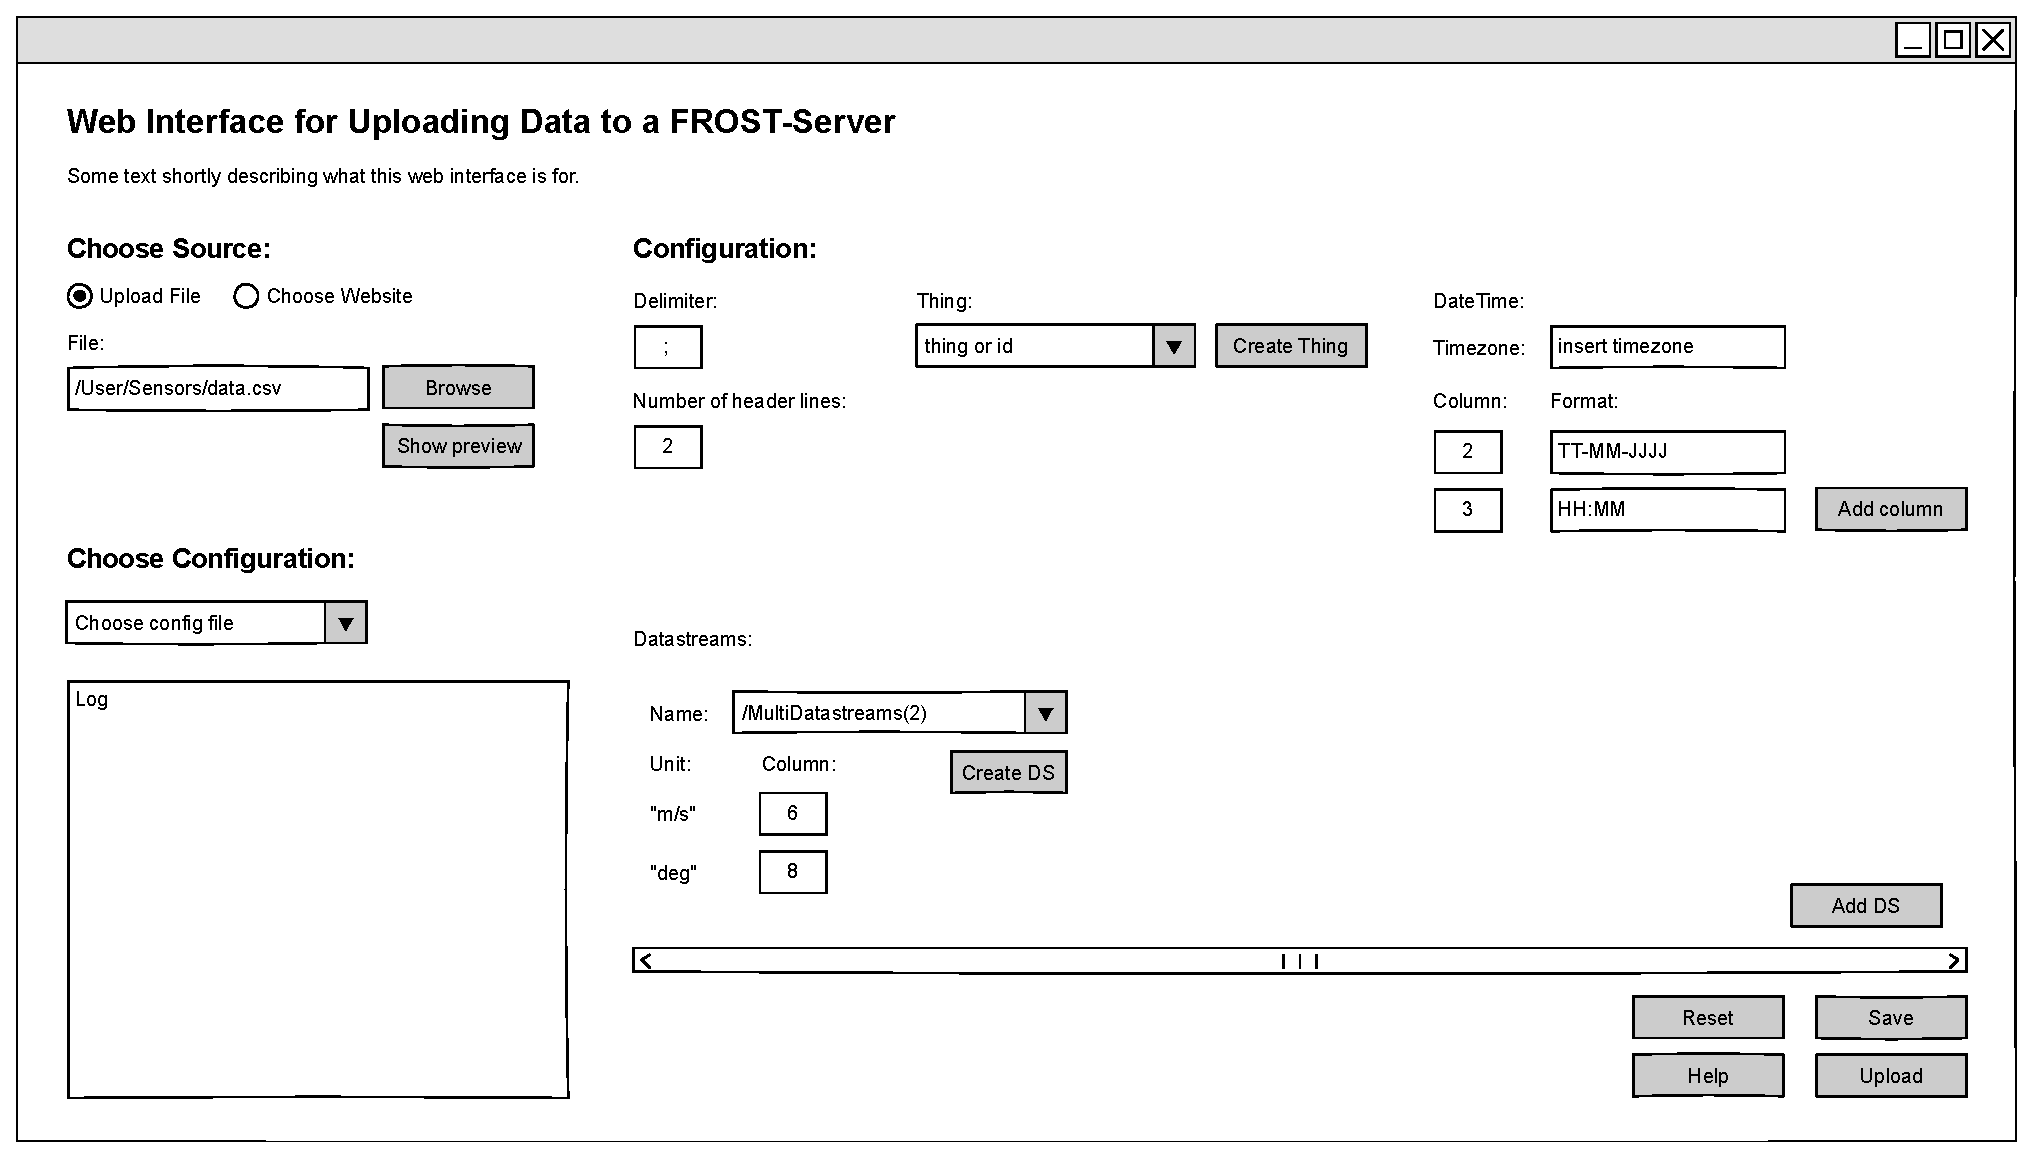
\includegraphics[scale=0.4]{images/gui}
\caption{\label{fig:guiMain}Hauptseite der Weboberfläche}
\end{figure}
Beim Aufrufen der Weboberfläche ist zu Beginn nur der Bereich zum Auswählen der Quelldatei sichtbar. 
Nach dem Einstellen der Quelle wird das Dateiformat überprüft und ein passender Konfigurator für das Spaltenformat der Datei und das Format der Daten in den Spalten wird sichtbar. \\

Über das Log werden eventuelle Fehlermeldungen und Übertragungsfortschritte angezeigt. Unter "{Choose Configuration}" lässt sich eine auf dem Server gespeicherte Konfigurationsdatei auswählen. Dort bieten sich folgende Möglichkeiten:
\begin{itemize}
\item Unter "{Configuration}" kann eingestellt werden, in welcher Form die Daten in der Quelldatei angespeichert sind, um diese dann in den vom FROST-Server verwendeten OGC-Standard zu konvertieren.
\item Zuerst ist das Trennsymbol für die Spalten in der Quelldatei und die Anzahl der Kopfzeilen (nicht zum Datensatz gehörige Zeilen) anzugeben. 
\item Dann kann das zu den Daten gehörige Thing von schon auf dem FROST-Server existierenden Things ausgewählt werden. Falls es benötigt wird, lässt sich über den "{Create Thing}"{-Button} ein neues Thing erstellen. (siehe \cref{fig:thing})
\item Unter "{DateTime}"{ ist} das Datumsfomat einstellbar. Erst wird die Zeitzone eingegeben und danach lassen sich das Format für das Datum bzw. die Zeit als RegEx und die zugehörige Spaltennummer angeben.
\item Abschließend lassen sich ein oder mehrere (Multi-)Datastreams auswählen. Existiert der (Multi-)Datastream noch nicht, kann er über "{Create DS}"{ erstellt} werden. Mit Hilfe des "{Add DS}"{-Buttons} lassen sich weitere (Multi-)Datastreams hinzufügen. Anschließend lassen sich wieder die zu den Daten gehörigen Spalten in der Quelldatei einstellen.
\item Außerdem bietet die Weboberfläche über den "{Save}"{-Button} die Möglichkeit, eine bestehende Konfiguration auf dem Server abzuspeichern bzw. über den "{Reset}"{-Button} auf die Standard-Konfiguration zurückzusetzen.
\item Über den "{Upload}"{-Button} werden die Daten auf den FROST-Server hochgeladen.
\item Der "{Help}"{-Button} ermöglicht den Zugriff auf eine Kurzanleitung für das Webinterface.
\end{itemize}

\subsection{Thing erstellen}
Wie in \cref{fig:thing} dargestellt, müssen Name, Beschreibung und Eigenschaften gewählt werden, um ein Thing zu erstellen. Über den "{Add property}"{-Button} kann eine weitere Eigenschaft als Key-Value-Paar hinzugefügt werden. Abschließend muss eine bestehende Location gewählt werden bzw. eine neue erstellt werden (siehe \cref{fig:loc}).

\begin{figure}[htbp]
\centering
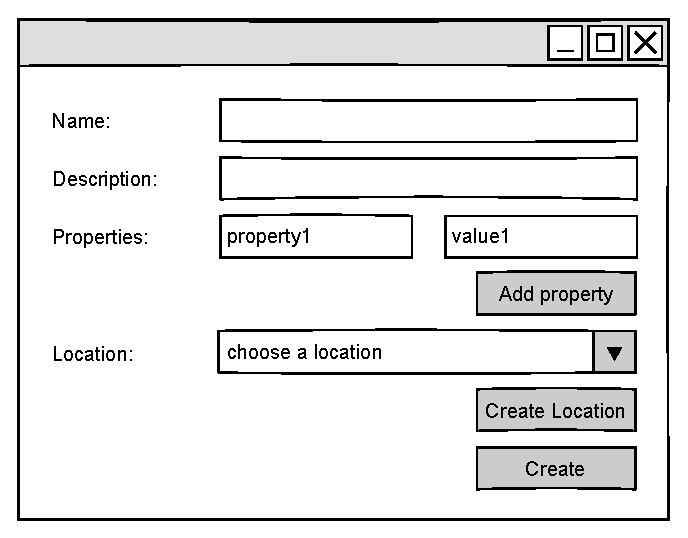
\includegraphics[scale=1]{images/thing}
\caption{\label{fig:thing}Dialogfenster zum Erstellen eines Things.}
\end{figure}


\subsection{Datastream erstellen}
\cref{fig:ds} zeigt das Dialogfenster zum Erstellen eines (Multi-)Datastreams. Es müssen erst Name, Beschreibung, Observation Type und ein Sensor gewählt werden. Soll dafür ein neuer Sensor angelegt werden, existiert der "{Create Sensor}"{-Button} (siehe \cref{fig:sensor}).\\

Im unteren Teil lassen sich die gemessenen Größen für eine Messwertreihe festlegen. Existiert eine solche Größe noch nicht, lässt sie sich über den "{Create Property}"{-Button} anlegen (siehe \cref{fig:oprop}). Mit dem "{Add unit}"{-Button} kann eine weitere Messwertreihe hinzugefügt werden. Hat ein Datastream mehr als eine solche Größe, wird er als MultiDatastream verwaltet.

\begin{figure}[htbp]
\centering
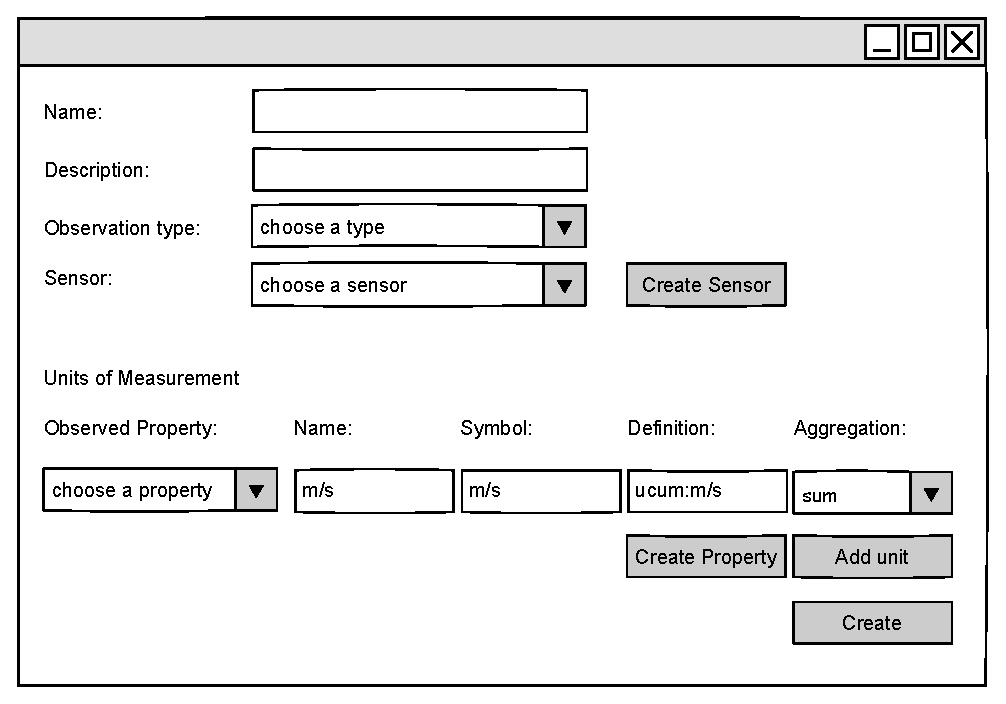
\includegraphics[scale=1]{images/datastream}
\caption{\label{fig:ds}Dialogfenster zum Erstellen eines Datastreams.}
\end{figure}

\subsection{Sensor, ObservedProperty oder Location erstellen}
Das Erstellen eines Sensors (siehe \cref{fig:sensor}), einer ObservedProperty (siehe \cref{fig:oprop}) oder einer Location (siehe \cref{fig:loc}) verläuft, indem alle Textfelder des jeweiligen Dialogfeldes passend ausgefüllt werden und anschließend der "{Create}"{-Button} gedrückt wird.

\begin{figure}[htbp]
\centering
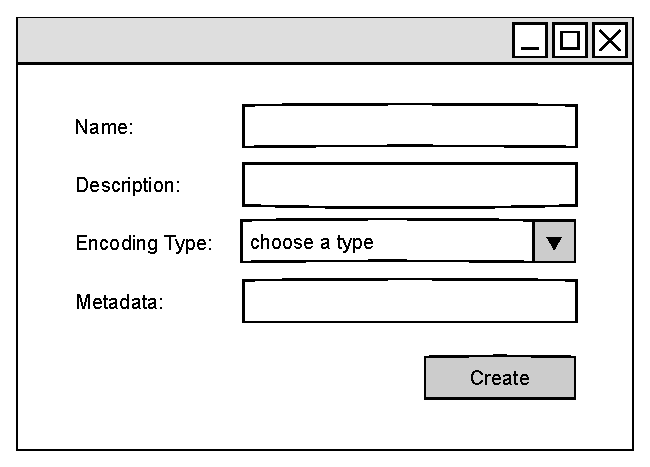
\includegraphics[scale=1]{images/sensor}
\caption{\label{fig:sensor}Dialogfenster zum Erstellen eines Sensors.}
\end{figure}

\begin{figure}[htbp]
\centering
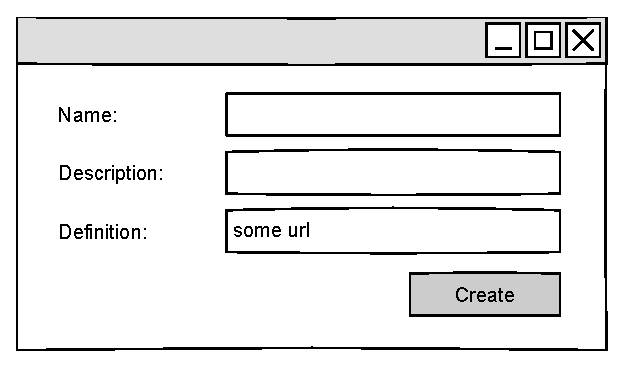
\includegraphics[scale=1]{images/oprop}
\caption{\label{fig:oprop}Dialogfenster zum Erstellen eines Things.}
\end{figure}

\begin{figure}[htbp]
\centering
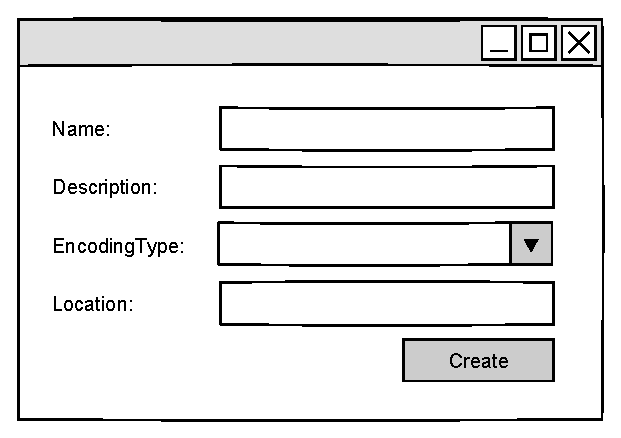
\includegraphics[scale=1]{images/loc}
\caption{\label{fig:loc}Dialogfenster zum Erstellen einer Location.}
\end{figure}
	
	\subsection{Erforderliche Funktionale Anforderungen}
	
	\begin{enumerate}
		\item Auswahlmöglichkeit der Datenquelle
		\begin{itemize}
			\item eine Datei
			\item externer Server (optional)
		\end{itemize}
		
		\item Laden, speichern von Konfigurationen
		
		\item Erstellen von Konfigurationen
		\begin{itemize}
			\item Einstellen der Datumsspalte/n
			\item Format des Datums einstellen
			\item Auswählen und erstellen von
			\begin{itemize}
				\item Things
				\item Locations, für neue Things
				\item Datastreams
				\item Sensors, für neue Datastreams
				\item Propertys, für neue Datastreams
			\end{itemize}
			\item Spaltenauswahl für Datenextraktion
		\end{itemize}
		
		\item Bereitstellen einer Default-Konfiguration
		
		\item Auswahlmöglichkeit des Zielservers
		\begin{itemize}
			\item Nicht in Webinterface möglich
		\end{itemize}
		
		\item Hochladen der Daten auf den Frost-Server
		
		\item Formatieren der Daten in OGC SensorThings API Standard
		
		\item Fehlermeldungen im Log
		\begin{itemize}
			\item Fehler in Datenzeilen
			\item Verbindungsfehler zum Frostserver
			\item Fehlerhafte Quelldatei
		\end{itemize}
		
		\item Anlegen einer Log-Datei mit
		\begin{itemize}
			\item Historie von Uploads
			\item Fehlermeldungen
		\end{itemize}
		
		\item Kurzanleitung auf der Weboberflächen.
	\end{enumerate}
	
	\subsection{Gewünschte Funktionale Anforderungen}
	\begin{enumerate}
		\item Duplikaterkennung um Datenredundanz zu vermeiden
		
		\item Rückgabe von Fehlerhaften Zeilen in einer neuen CSV-Datei
		
		\item Auswahlmöglichkeit komplexer Operationen auf Daten:
		\begin{itemize}
			\item Summe
			\item Minimum
			\item Maximum
			\item Durchschnitt
		\end{itemize}
		Operationen sind nur Spaltenweise  möglich. 
	\end{enumerate}

	%TODO Nummerierung der Wunschkriterien in Fließtext
	\subsection{Produktdaten}
	
	Bei den Daten die auf dem Server gespeichert werden müssen wird unterschieden zwischen Nutzerdaten und Systemdaten.
	
\begin{itemize}
	\item Nutzerdaten:
	\begin{itemize}
		\item Konfigurationen
	\end{itemize}
	\item Systemdaten:
	\begin{itemize}
		\item Log-Datei
		\item Adresse des FROST-Servers
		\item Adresse der entfernten CSV/XLSX - Datei (optional) 
	\end{itemize}
\end{itemize}
	
	\subsection{Produktleistungen}
	\begin{itemize}
		\item Die Software dokumentiert Fehler jeglicher Art und das starten b.z.w abschließen von Uploads.
		\item Die Eingaben werden direkt verarbeitet. Dem Nutzer wird sofort Feedback über eine Fortschrittsleiste gegeben, sollte die Anfrage länger als eine Sekunde dauern.
		\item Die Daten werden korrekt an den FROST-Server übermittelt, dazu gehört auch Robustheit der Anwendung gegenüber falschen Angaben.
		\item Der Nutzer erhält bei falschen Angaben oder Fehlern eine Rückmeldung.
	\end{itemize}
	
	
	\subsection{Qualitätsanforderungen}
	Backend-Anforderungen (Software) :
	\begin{itemize}
	\item Das Programm soll über lange Zeiträume auch ohne Unterbrechungen zuverlässig ausgeführt werden können, solange die Produktumgebung dies zulässt.
	\item Interaktion oder Beobachtung durch den Nutzer werden nicht vorrausgesetzt.
	\item Eine einfache Portierung ist gegeben, da die Software auf Java basiert und damit Platformunabhängig ist. 
	\item Zu große oder zu viele Anfragen werden abgelehnt um Sicherheit zu gewährleisten und einer Überlastung des Servers vorzubeugen.
	\item Es soll möglichst einfach sein die Software schnell und unkompliziert zu ändern oder zu erweitern.
	\end{itemize}
	Frontend-Anforderungen (Weboberfläche) :
	\begin{itemize}
	\item Die Benutzbarkeit hat höchste Priorität, auch Nutzer ohne oder wenig technischem Vorwissen sollen in der Lage sein die Software zu bedienen.
	\item Die Daten sollten HTTPS-/SSL-Verschlüsselt werden um Abfangen der Daten zu verhindern.
	\end{itemize}
	
	\subsection{Anwendungsszenarien}
	Ideen für Anwendungsszenarien:
	%TODO Anwendungsfalldiagramm
	\begin{itemize}
		\item Nutzer ohne technische Kenntnisse des Frost Server Aufbaus besitzt einen Frost Server und einen Sensor, der schon auf dem Frost Server abgespeichert ist. Außerdem hat er eine csv-Datei mit Daten vom Sensor, der einen schon bestehenden Datensatz des Sensors auf dem Server erweitern soll. Er navigiert in seinem Browser zur Web-oberfläche und stellt seine Datei als Quelle und den Frost Server als Ziel ein. Dann wählt er eine Favoritenkonfiguration aus, die zu seinem Sensor passt und lädt seine Daten durch Klick des "Upload"-Buttons hoch. Die Daten werden formatiert und auf dem Server abgespeichert.
		\item das gleiche mit einem erfahrenen Nutzer, der ein neues Thing, einen Sensor und zugehörigen Datastream erstellt
		\item Szenario zum Abspeichern einer Konfiguration
	\end{itemize}
	
	
	\subsection{Testfälle}
	\test{Default Case zum }{}
	
	\test{Anzeigen der Weboberfläche}{}
	\ \\
	\teststep{Der Nutzer hat einen Browser geöffnet.}{Der Nutzer navigiert auf die Webseite.}{Die Webseite wird wie in \cref{fig:guiMain} dargestellt.}
	\ \\
	\test{Datei als Quelle wählen}{}
	\ \\
	\teststep{Dem Nutzer wird die Webseite angezeigt.}{Der Nutzer wählt die Radio-Box "{Upload File}".}{Es wird ein Textfeld und ein "Browse\string"\string-Knopf angezeigt, um die hochzuladende Datei festzulegen.}
	\ \\
	\teststep{}{Der Nutzer drückt den "{Browse}"{-Knopf}.}{Es öffnet sich ein Dateimanager zum Auswählen der Datei.}
	\ \\
	\teststep{}{Der Nutzer wählt seine Datei aus.}{Der Dateipfad erscheint im Textfeld.}
	\ \\
	\test{Entfernte Webseite als Quelle wählen}{}
	\ \\
	\teststep{Dem Nutzer wird die Webseite angezeigt.}{Der Nutzer wählt die Radio-Box "{Choose Website}".}{Es wird ein Textfeld angezeigt, um die URL der entfernten Webseite festzulegen.}
	\ \\
	\teststep{}{Der Nutzer gibt eine URL ein.}{Die URL wird auf Gültigkeit überprüft und die zu ladende Datei auf dem Server der Weboberfläche zwischengespeichert.}
	\ \\
	\test{Zielserver wählen}{}
	\ \\
	\teststep{Dem Nutzer wird die Webseite angezeigt. Insbesondere existiert ein Textfeld zur Eingabe des Zielservers.}{Der Nutzer gibt einen FROST-Server als Ziel in das Textfeld ein und drückt den "{Submit}"{-Knopf}.}{Der Server wird auf Gültigkeit überprüft und bei Korrektheit erscheint ein Konfigurator zum Einstellen des Formats der Daten in der Quelldatei. Im Konfigurator ist der Default-Case voreingestellt.}
	\ \\
	\test{Konfiguration zurücksetzen}{}
	\ \\
	\teststep{Der Nutzer befindet sich auf der Webseite und es wird der Konfigurator angezeigt.}{Der Nutzer drückt den "{Reset}"{-Knopf}.}{Alle eingestellten Konfigurationen werden auf den Default-Case zurückgesetzt.}
	\ \\
	\test{Hilfe anfordern}{}
	\ \\
	\teststep{Der Nutzer befindet sich auf der Webseite.}{Der Nutzer drückt den "{Hilfe}"{-Knopf}.}{Es wird eine Anleitung für den Gebrauch der Weboberfläche angezeigt.}
	\ \\
	\test{Konfiguration abspeichern}{}
	\ \\
	\teststep{Der Nutzer hat eine Konfiguration erstellt.}{Der Nutzer drückt den "{Save}"{-Knopf}.}{Es wird eine cfg-Datei der Konfiguration erstellt und der Download der Datei wird angestoßen.}
	\ \\
	\test{Konfiguration laden}{}
	\ \\
	\teststep{Der Nutzer befindet sich auf der Webseite und hat eine gültige Quelldatei und einen gültigen Zielserver angegeben. Es wird ein Konfigurator angezeigt.}{Der Nutzer drückt den "{Browse}"{-Knopf}.}{Es öffnet sich ein Dateimanager.}
	\ \\
	\teststep{}{Der Nutzer wählt eine cfg-Datei.}{Die Datei wird auf Korrektheit überprüft und im Erfolgsfall ist der Konfigurator entsprechend der Datei eingestellt.}
	
	\ \\
	\test{Sensor erstellen}{}
	\ \\
	\teststep{Der Nutzer erstellt gerade einen Datastream (sieht den Dialog \ref{fig:ds}) und der zugehörige Sensor existiert noch nicht.}{Der Nutzer drückt den "{Create Sensor}"{-Knopf}.}{Es öffnet sich das Dialogfenster zum Erstellen eines Sensors (vgl \ref{fig:sensor}).}
	\ \\
	\teststep{}{Der Nutzer füllt alle Textfelder aus und drückt den "{Create}"{-Knopf}.}{Die Daten werden überprüft und ein neuer Sensor wird angelegt. Das Dialogfenster wird geschlossen.}
	
	\ \\
	\test{ObervedProperty erstellen}{}
	\ \\
	\teststep{Der Nutzer erstellt gerade einen Datastream (sieht den Dialog \ref{fig:ds}) und eine ObservedProperty für einen Datensatz existiert noch nicht.}{Der Nutzer drückt den "{Create Property}"{-Knopf}.}{Es öffnet sich das Dialogfenster zum Erstellen einer ObservedProperty (vgl \ref{fig:obsProp}).}
	\ \\
	\teststep{}{Der Nutzer füllt alle Textfelder aus und drückt den "{Create}"{-Knopf}.}{Die Daten werden überprüft und ein neue ObservedProperty wird angelegt. Das Dialogfenster wird geschlossen.}
	\ \\
	
	\test{Einen Datensatz zu einem Datastream hinzufügen}{}
	\ \\
	\teststep{Der Nutzer erstellt gerade einen Datastream (sieht den Dialog \ref{fig:ds}).}{Der Nutzer drückt den "{Add unit}"{-Knopf}.}{Es wird eine neue leere Zeile in der Tabelle für die zum Datastream gehörigen Units of Measurement angelegt.}														  			   
	
	
	\test{Einstellen nichts neu}{}
	\teststep{Der Nutzer hat Quelle und Ziel eingegeben und bestätigt}{Der Nutzer füllt die Datums-/Uhrzeits-Spalte aus}{Die Software überprüft die Korrektheit der Spalten (Wurde eine Spalte angegeben, die nicht existiert?)}
	\teststep{Die Spalten wurden korrekt angegeben}{Der Benutzer gibt via RegEx das Format des Datums/der Uhrzeit in dem dazugehörigen Textfeld an}{Die Korrektheit des RegEx wird anhand der Werte der Tabellendatei auf Fehler geprüft}
	\teststep{Das Datum / die Uhrzeit wurde korrekt ausgefüllt}{Der Nutzer wählt das Thing aus dem Dropdown-Menü, welches alle Things enthält, aus}{Das Datastream-Dropdown-Menü wird mit den zum gewählten Thing gehörenden Data-/MultiData-Streams aktualisiert}
	\teststep{Thing wurde ausgewählt}{Der Anwender wählt den Datastream aus dem Datastream-Dropdown-Menü aus}{Das System lädt die zum Datastream/MultiDataStream gehörenden Messeinheiten neben die Textfelder zum eintragen}
	\teststep{Messdaten geladen}{Der Nutzer trägt die Spalten mit den Messwerten neben die Messeinheiten ein}{Die Korrektheit der Eintragung wird wieder durch die Software geprüft}
	\teststep{Alle Textfelder ausgefüllt}{der User klickt auf den Button "{Upload}"}{Die Daten in den angegebenen Spalten werden eingelesen, konvertiert und auf den FROST-Server übertragen}
	
	\test{Neue Datums-/Zeit-Spalte erstellen}{}
	\teststep{Der Nutzer hat die Datei geladen und den Server angegeben, es wird keine CFG-Datei genutzt (Ende von Test 1-fach)}{Der Benutzer drückt den "+"-Button, um eine neue Datums-/Zeit-Spalte anzulegen}{Die Software erstellt zwei neue Textfelder mit "Spalte" und "Format" im Interface, sodass sich die Datums- und Zeitnagabe über mehrere Spalten erstrecken kann}
	
	\test{Datastream hinzufügen}{}
	\teststep{Ein Thing wurde ausgewählt, die Datastreams wurden in das Dropdown-Menü geladen}{Der Nutzer klickt auf den "{Add DS}"{-Button}}{Das Webinterface wird aktualisiert und rechts vom letzten Datastream wird ein neues Dropdown-Menü für einen neuen Datastream und neue Textfelder hinzugefügt}
	
	\test{Neues Thing erstellen}{}
	\teststep{Die Datei und die FROST-Server-Domain wurden angegeben/hochgeladen}{Der Nutzer klickt auf den "{Create Thing}"{-Button}}{es öffnet sich der "{Create New Thing}"{-Dialog}}
	\teststep{Das Dialogfenster ist offen, Name und Beschreibung des Things wurden in die Textfelder eingetragen, die Location wurde aus dem Dropdown-Menü ausgewählt}{Der Nutzer klickt auf "{Create}"}{Das Thing wird auf dem FROST-Server erstellt und in dem Hauptinterface dem Dropdown-Menü hinzugefügt}
	
	\test{Properties hinzufügen}{}
	\teststep{Der "{Create New Thing}"{-Dialog} ist offen}{Der Nutzer klickt einmal oder mehrfach auf den "{Add Property}"{-Button}}{es werden ein oder mehrere Textfeld-Paare im Interface erstellt in denen der Nutzer die Eigenschaft (Property) und den Wert (Value) des Things einstellen kann}
	
	\test{Neuen (Multi)DataStream erstellen}{}
	\teststep{Die Datei und FROST-Server wurden angegeben und ein Thing ausgewählt}{Der User klickt auf den "{Create DS}"{-Button}}{Es öffnet sich der "{Create New DataStream}"{-Dialog} indem der User einen neuen DataStream oder MultiDataStream formulieren und erstellen kann}
	\teststep{Der User sieht das Dialogfenster zum erstellen eines DataStreams}{der User trägt Name und Beschreibung in die Textfelder ein, wählt Observation Type und Sensor aus den Dropdown-Menüs aus, trägt eine oder mehrere Units Of Measurement ein und klickt abschließend auf "{Create}"}{Die Software unterscheidet zwischen DataStream und MultiDataStream und legt den entsprechenden Stream mit den angegeben Daten im FROST-Server an}
	
	
	\subsection{Zeitplanung}
	Beispielhafte Terminplanung: \\
	\begin{itemize}
		\item 07.05. - 27.05.: Pflichtenheft
		\item 28.05. - 24.06.: Entwurfsphase
		\item 25.06. - 22.07.: Implementierung
		\item 23.07. - 12.08.: Beispiel-Urlaubstermin (2 Wochen)
		\item 13.08. - 02.09.: Qualitätssicherung
		\item 03.09. - 09.09.: Terminfenster interne Abnahme
		\item 10.09. - 17.09.: Terminfenster Abschlusspräsentation
	\end{itemize}
	
	
	\subsection{Glossar}
	\begin{itemize}
		\item FROST \\
		Der \textbf{FR}auenhofer \textbf{O}penSource \textbf{S}ensor\textbf{T}hings-Server ist die erste komplette quelloffene Implementierung der OGC SensorThings API
		\item OGC \\
		Das \textbf{O}pen \textbf{G}eospatial \textbf{C}onsortium ist eine gemeinnützige Organisation, die sich zum Ziel gesetzt hat, die Entwicklung von raumbezogener Informationsverarbeitung (insbesondere Geodaten) auf Basis allgemeingültiger Standards festzulegen.
		\item SensorThings API \\
		Allgemeiner einheitlicher Standard um Verbindung zwischen Sensoren, deren Ort und Umgebung und den von ihnen erzeugten Daten herzustellen.
		\item CSV-/XLSX-Dateien \\
		CSV (Comma Seperated Value, .csv) und Excel (.xlsx) sind gängige Dateiformate zum Speichern von Daten (hier speziell: Sensor-Daten) in Tabellenform.
		\item CFG-Datei \\
		Konfigurationsdateien(kurz: CFG-Dateien) sind Textdateien, die speziell zur Speicherung bestimmter Einstellungen (Konfigurationen) dienen.
		\item Thing \\
		Ein Thing (deutsch: Ding) ist nach Definition der SensorThings API ein Objekt der physischen oder virtuellen Welt. Es benötigt einen Namen und eine Beschreibung. Es können sich ein oder mehrere Datastreams auf ein Thing beziehen.
		\item Datastream \\
		Ein Datastream ist eine fortlaufende Sammlung von Messungen (Observations) des selben Sensors.
		\item Integer \\
		Mit Integer wird in der Informatik ein Datentyp bezeichnet, der ganzzahlige Werte speichert.
		\item NULL \\
		Als Nullwert (kurz NULL) bezeichnet man in der Informatik einen Zustand, der das Fehlen eines Wertes anzeigen soll.
		\item Magic Numbers \\
		Deutsch: Magische Zahl. Ein im Quellcode eines Programms auftauchender Zahlenwert, dessen Bedeutung sich nicht unmittelbar erkennen lässt.
		\item Log-Datei \\
		Eine Log-Datei, auch Protokoll-Datei, enthält das automatisch geführte Protokoll aller oder bestimmter Aktionen von Prozessen auf einem Computersystem.
		\item Docker \\
		Docker ist eine Software zur Isolierung von Anwendungen. Docker vereinfacht die Bereitstellung von Anwendungen, weil sich sog. Container, die alle nötigen Pakete enthalten, leicht als Dateien transportieren und installieren lassen.
		\item GUI \\
		Ein Grafische Benutzeroberfläche (engl. \textbf{G}raphical \textbf{U}ser \textbf{I}nterface) hat die Aufgabe, eine Anwendungssoftware auf einem Rechner mittels grafischer Symbole und Steuerelemente für den Benutzer bedienbar zu machen.
		\item (Java) JRE \\
		Mit der Java-Laufzeitumgebung (\textbf{J}ava \textbf{R}untime \textbf{E}nvironment) werden Programme (Java-Anwendungen) weitgehend unabhängig vom darunter liegenden Betriebssystem ausgeführt.
		\item JavaScript \\
		JavaScript ist eine Programmiersprache, die hauptsächlich auf Webbrowsern Anwendung findet.
		\item headless Server \\
		Als headless (kopflos) bezeichnet man Computer, meist Serversysteme, die über keinen Bildschirm oder sonstige grafische Ausgabe verfügen.
		Diese Systeme haben als Steuerungsmöglichkeit in vielen Fällen eine Netzwerkverbindung.
		\item README \\
		Als README (deutsch: Liesmich) wird eine Datei bezeichnet, die üblicherweise mit Software mitgeliefert wird und diverse, oft wichtige Informationen über die Software enthält.
		\item Regex \\
		\textbf{Reg}ular \textbf{Ex}pressions (Regex, regulärer Ausdrucke) dienen der Beschreibung von Zeichenketten mit ähnlichem Format.
		Sie können als Filterkriterien in der Textsuche verwendet werden, indem der Text mit dem Muster des regulären Ausdrucks verglichen wird.
		\item HTTPS/SSL \\
		\textbf{H}yper\textbf{T}ext \textbf{T}ransfer \textbf{P}rotocol \textbf{S}ecure (HTTPS) ist ein sicheres Hypertext-Übertragungsprotokoll, das SSL benutzt.
		SSL steht für \textbf{S}ecure \textbf{S}ockets \textbf{L}ayer und ist die Standardtechnologie für die Absicherung von Internetverbindungen und den Schutz sensibler Daten, die zwischen zwei Systemen übertragen werden.
		\item GPLv3 \\
		GPLv3 ist die aktuelle Version von GPL. Diese \textbf{G}eneral \textbf{P}ublic \textbf{L}icense (allgemeine Veröffentlichungsgenehmigung) ist die am weitesten verbreitete Softwarelizenz,
		die einem gewährt, die Software auszuführen, zu studieren, zu ändern und zu verbreiten.
	\end{itemize}
	
\newpage
\subsection{Anhang}

\begin{textblock*}{\paperwidth}(0mm,0.2\paperheight)
\begin{figure}[t]
\centering
\noindent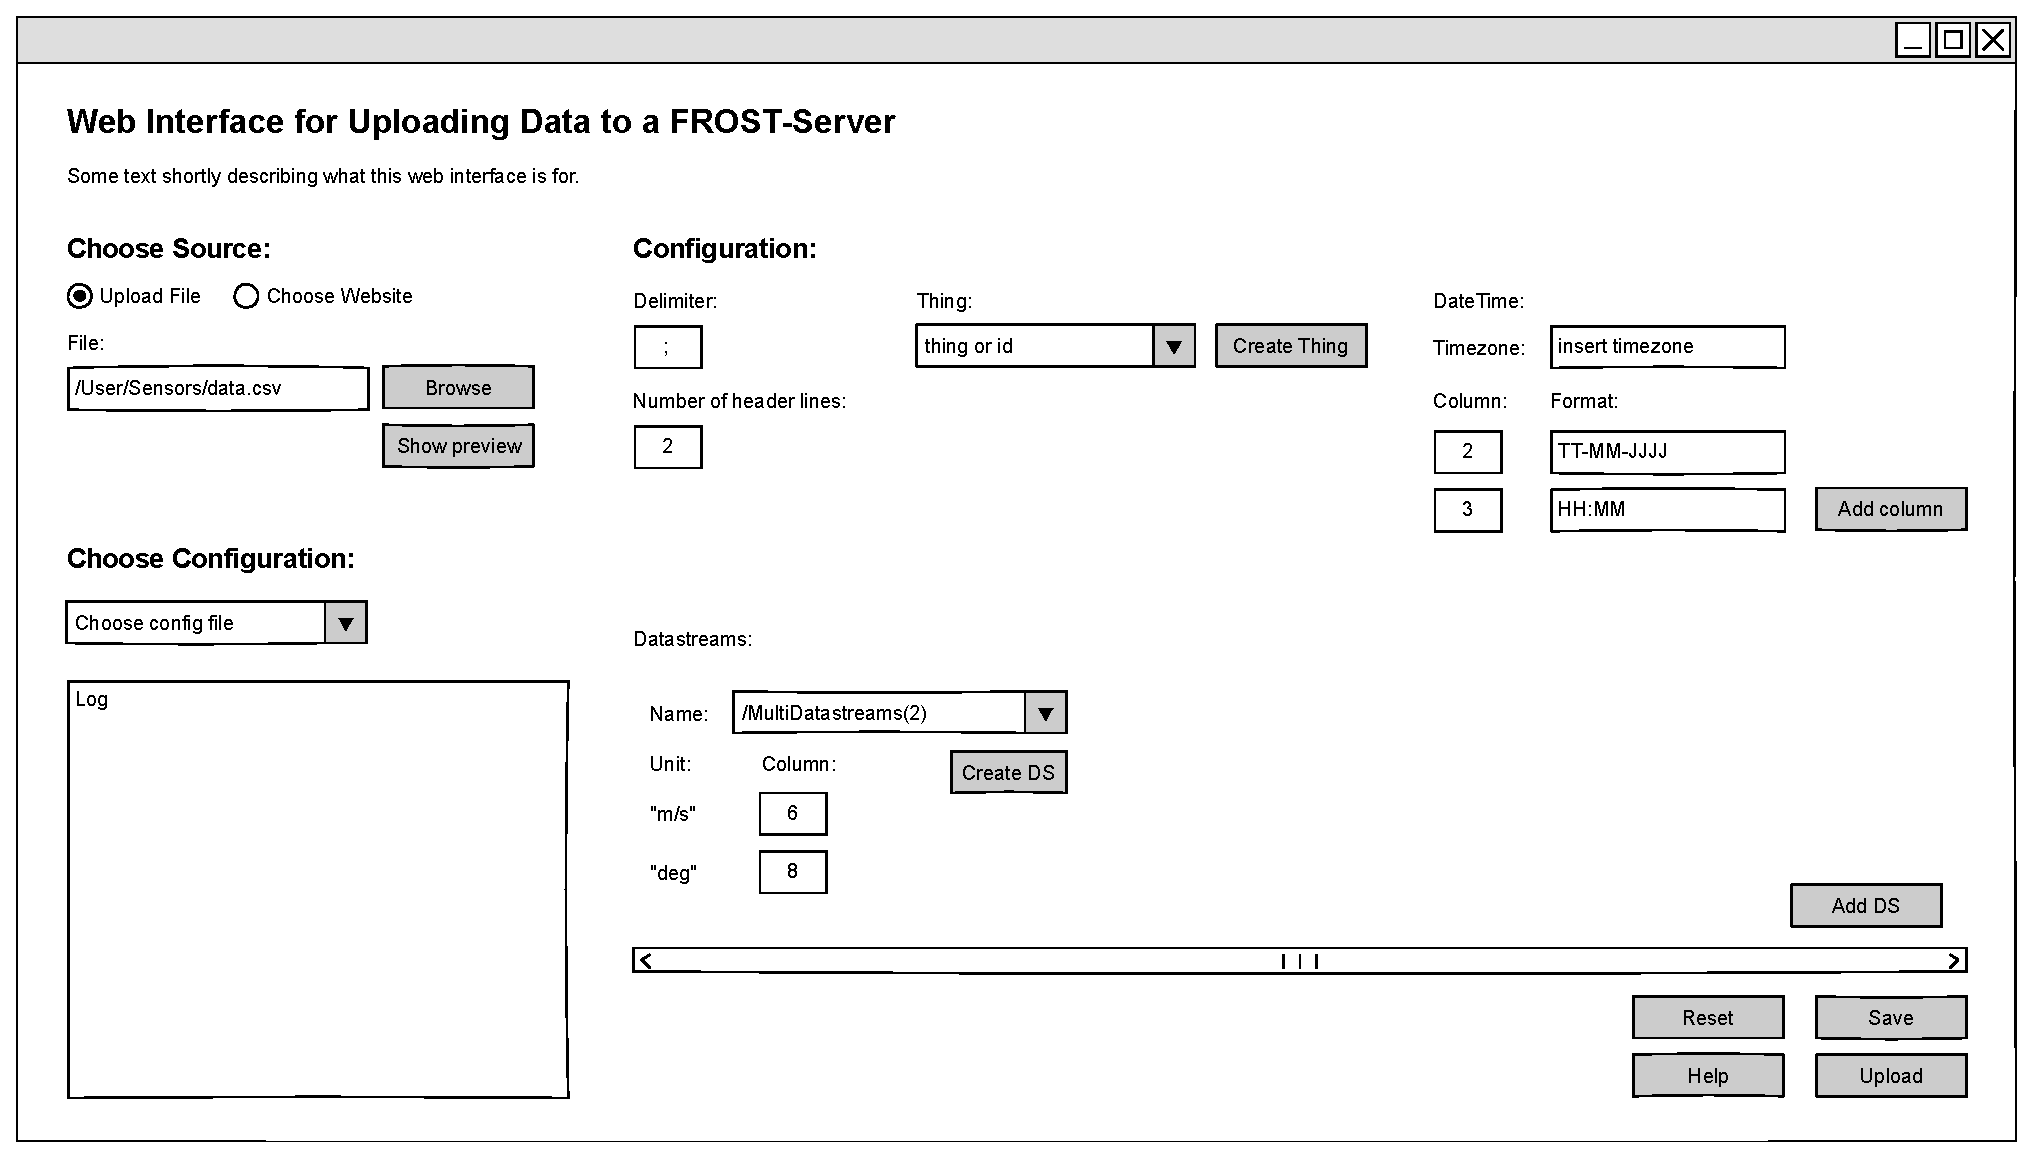
\includegraphics[scale=0.5, angle=90]{images/gui}
\caption{\label{fig:guiMainA}Hauptseite der Weboberfläche}
\end{figure}
\end{textblock*}
	
\end{document}
